\documentclass[a4paper,12pt]{jsarticle}

% 数式
\usepackage{amsmath,amsfonts}
\usepackage{bm}
\usepackage{enumerate}

% 画像
\usepackage[dvipdfmx]{graphicx}
\usepackage{here}

\usepackage{listingsutf8,jlisting} %日本語のコメントアウトをする場合jlistingが必要
%ここからソースコードの表示に関する設定
\lstset{
  basicstyle={\ttfamily},
  identifierstyle={\small},
  commentstyle={\smallitshape},
  keywordstyle={\small\bfseries},
  ndkeywordstyle={\small},
  stringstyle={\small\ttfamily},
  frame={tb},
  breaklines=true,
  columns=[l]{fullflexible},
  numbers=left,
  xrightmargin=0zw,
  xleftmargin=3zw,
  numberstyle={\scriptsize},
  stepnumber=1,
  numbersep=1zw,
  lineskip=-0.5ex
}

\begin{document}

\title{最適化1追加レポート}
\author{坪井正太郎(101830245)}
\date{\today}
\maketitle

\section{期末試験}

\subsection*{(1)2段階シンプレックス法}
\subsubsection*{1.}
\[\bm{x}_B=\bm{A}^{-1}\bm{b}, \bm{x}_N=\bm{0}\]

\subsubsection*{2.}
(B)の最適解を目的関数に代入した値が、
\begin{enumerate}[(i)]
  \item 0のとき$\rightarrow $その時の基底解が、元の問題(A)の実行可能解となる。
  \item 0でないとき$\rightarrow $(A)に実行可能解が存在しない。
\end{enumerate}

\subsection*{(2)双対性}
\subsubsection*{1.}
\begin{align*}
  目的関数:\quad & 12w_1 + 20w_2 \rightarrow 最大 \\
  制約条件:\quad & w_1 + w_2 \leq -2              \\
                 & 2w_1+4w_2\leq -1               \\
                 & 2w_2\leq -1
\end{align*}

\subsubsection*{2.}

$\bm{c}^T\bm{x}^*>=\bm{b}^T\bm{w}$となるような(D)の実行可能解$\bm w$のうち、最大なのは$\bm w^*$であり、$\bm w^*$が(D)の最適解である。
同時に、$\bm c^T\bm x>=\bm b^T\bm w^*$となるような(P)の実行可能解$\bm x$のうち、最小なのは$\bm x^*$であり、$\bm x^*$が(P)の最適解である。

\subsection*{(3)最適化1}
\section{}
最適化の授業の中で、塗り分け問題の定式化について最も興味を持った。
このような地図の塗り分け問題があることは、知っていたが、愚直解を求める以外の方法を知らなかった。
整数問題として定式化する方法があるという方法、0-1変数の導入が知れた点が良かった。

\section{期末レポート}
\subsection{シンプレックス法}
\subsubsection*{(a)}
\begin{figure}[H]
  \centering
  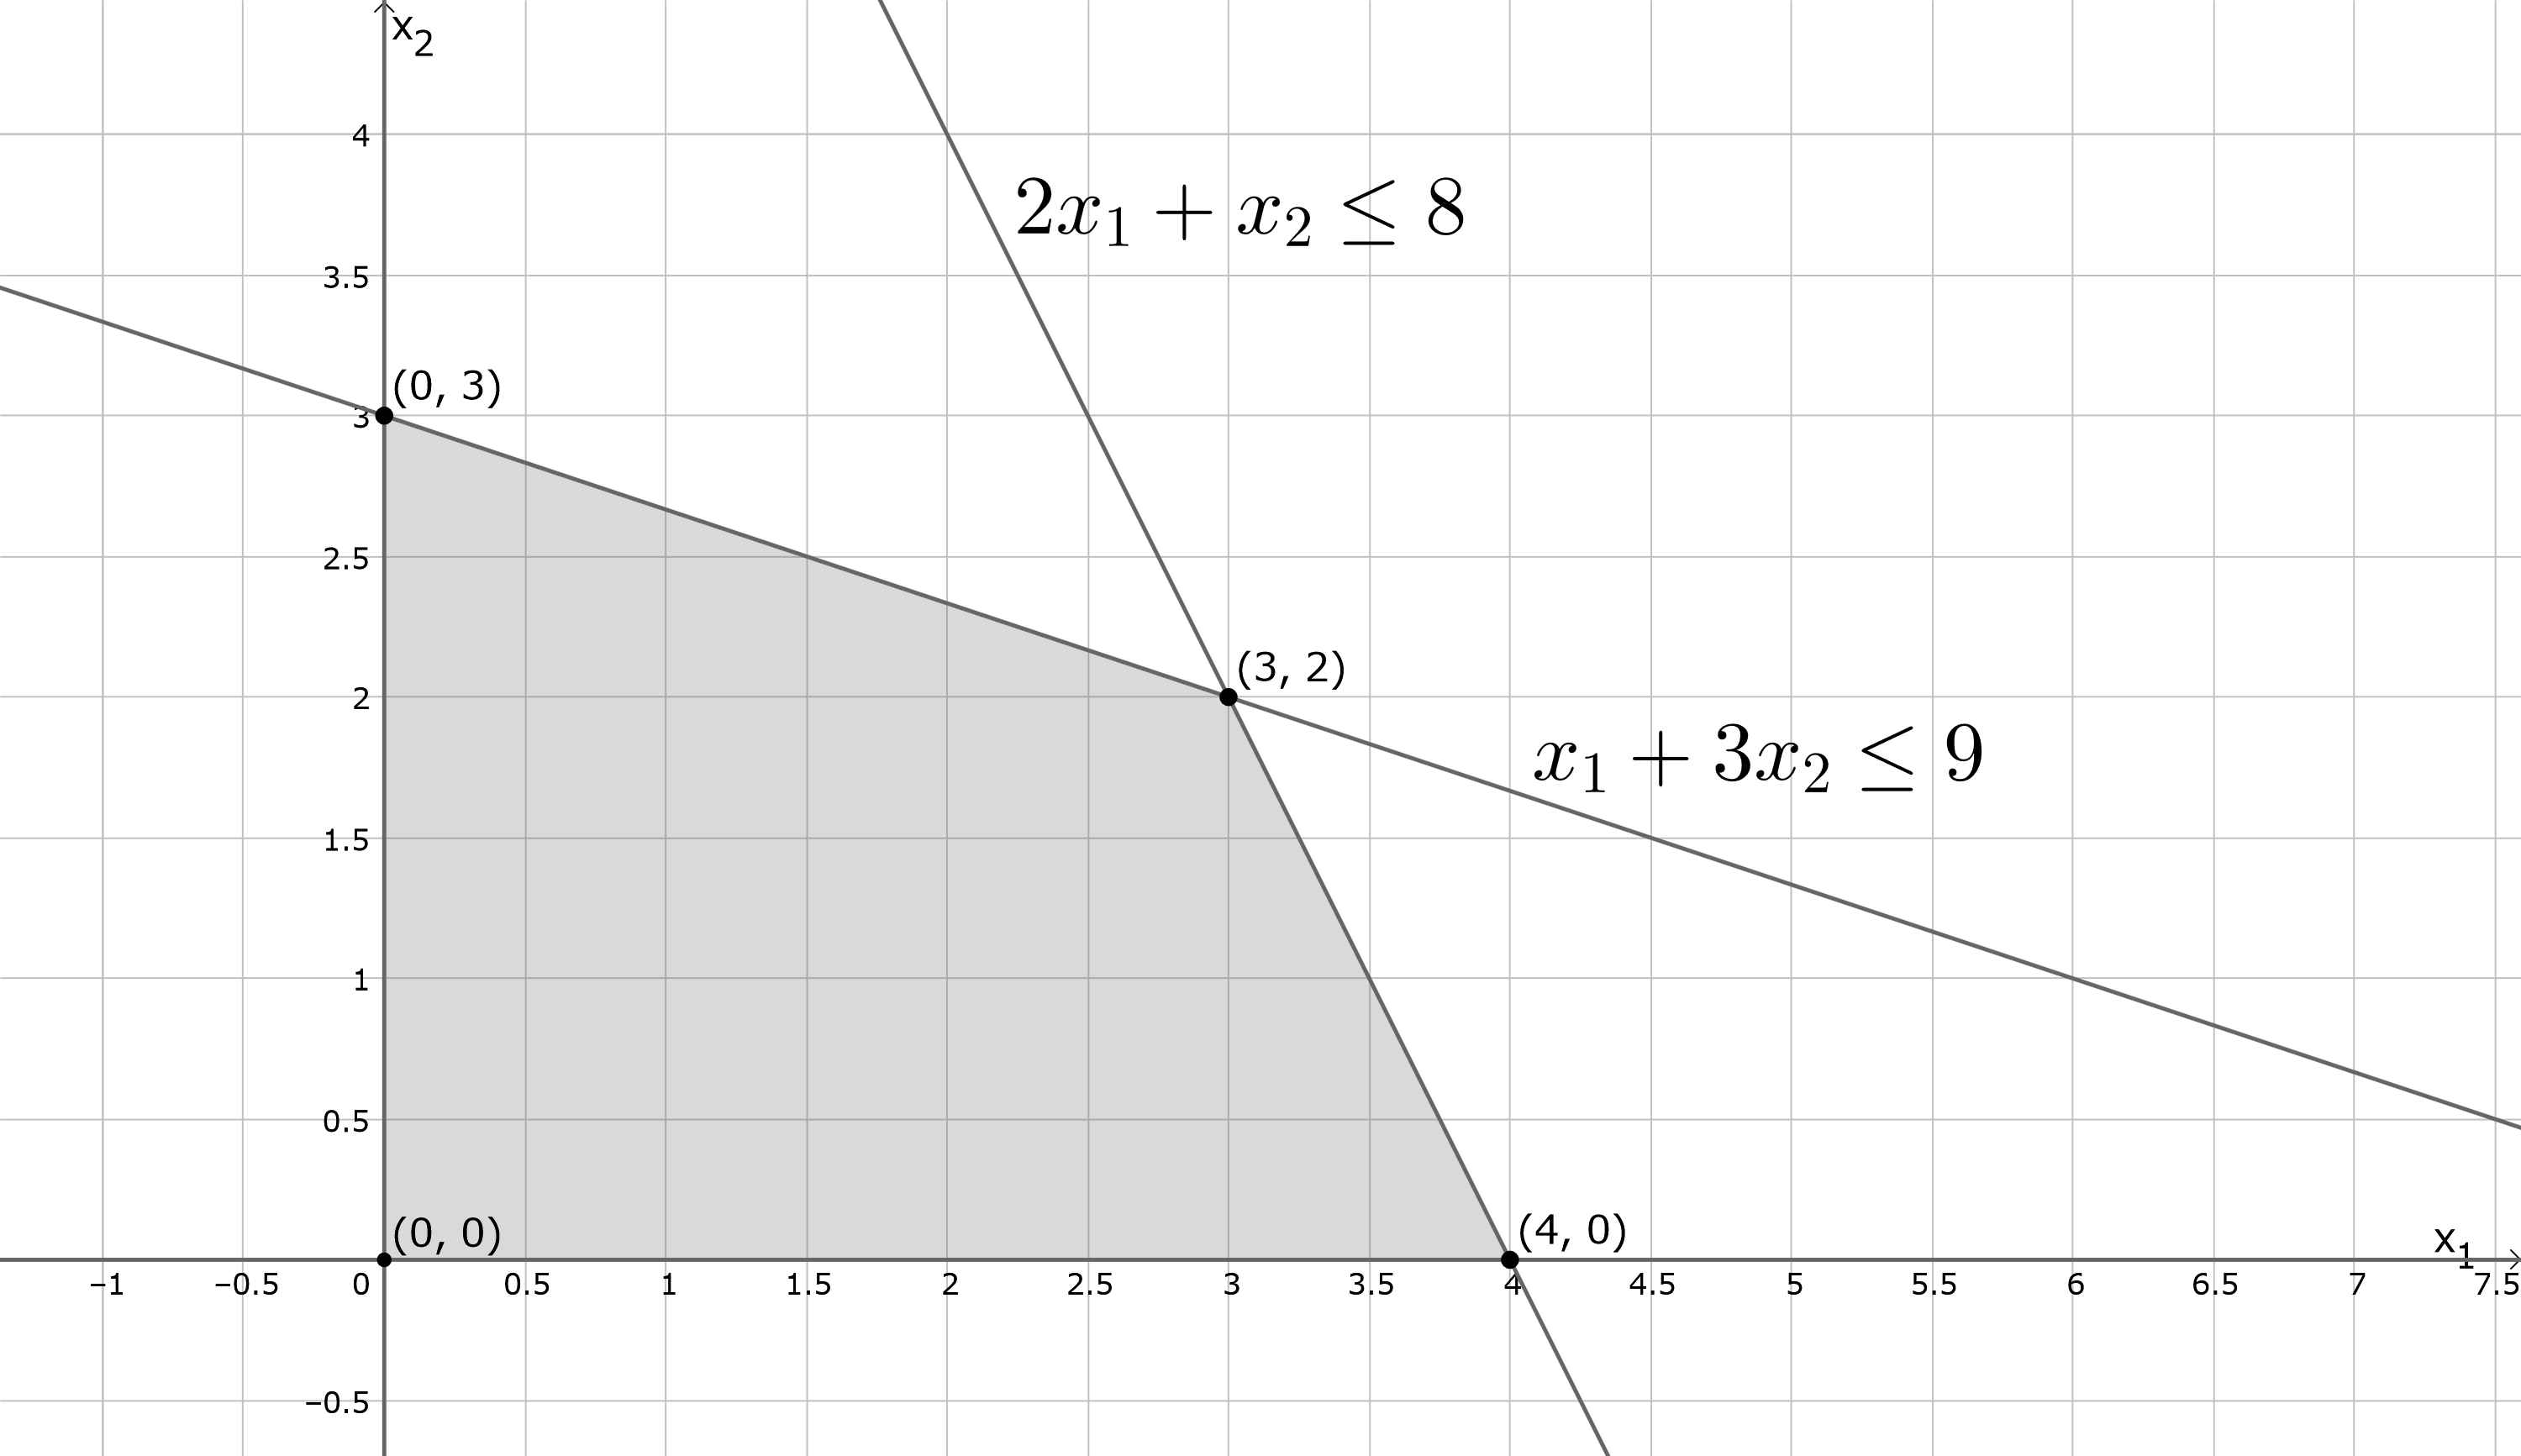
\includegraphics[width=13cm]{01.png}
  \caption{実行可能領域}
  \label{実行可能領域}
\end{figure}

\subsubsection*{(b)}
\begin{align*}
  目的関数:\quad & -2x_1-3x_2 \rightarrow 最大 \\
  制約条件:\quad & 2x_1+x_2+x_3 = 8            \\
                 & x_1+3x_2+x_4 = 9            \\
                 & x_1,x_2,x_3,x_4\geq 0
\end{align*}

\subsubsection*{(c)}
まず、初期条件は次のようになる。
\[
  \bm{B}=
  \begin{pmatrix}
    1 & 0 \\
    0 & 1
  \end{pmatrix}
  ,\bm{N}=
  \begin{pmatrix}
    2 & 1 \\
    1 & 3
  \end{pmatrix}
  ,\bm{c}_B=
  \begin{pmatrix}
    0 \\ 0
  \end{pmatrix}
  ,\bm{c}_N=
  \begin{pmatrix}
    -2 \\ -3
  \end{pmatrix}
\]

\begin{enumerate}
  \item
        \begin{enumerate}
          \item \[\pi =(\bm{B}^T)^{-1}\bm{c}_B=
                  \begin{pmatrix}
                    0 \\0
                  \end{pmatrix}\]
          \item \[\bm{c}_N-\bm{N}^T\pi=
                  \begin{pmatrix}
                    -2 \\-3
                  \end{pmatrix}\]
          \item \[\bm{y}=\bm{B}^{-1}\bm{a}_1=
                  \begin{pmatrix}
                    1 \\3
                  \end{pmatrix}
                  ,\bar{\bm{b}}=
                  \begin{pmatrix}
                    8 \\9
                  \end{pmatrix}\]
          \item \[\theta =3\]
          \item \[\bm{x}_N=
                  \begin{pmatrix}
                    0 \\3
                  \end{pmatrix}
                  ,\bm{x}_B=
                  \begin{pmatrix}
                    5 \\0
                  \end{pmatrix}と更新されるので、
                  \bm{x}=
                  \begin{pmatrix}
                    0\quad 2\quad 5\quad 0
                  \end{pmatrix}^T\]
        \end{enumerate}
  \item
        \begin{enumerate}
          \item \[\pi =
                  \begin{pmatrix}
                    0 \\-1
                  \end{pmatrix}\]
          \item \[\bm{c}_N-\bm{N}^T\pi=
                  \begin{pmatrix}
                    -1 \\1
                  \end{pmatrix}\]
          \item \[\bm{y}=
                  \begin{pmatrix}
                    \frac{1}{3} \\\frac{5}{3}
                  \end{pmatrix}
                  ,\bar{\bm{b}}=
                  \begin{pmatrix}
                    3 \\5
                  \end{pmatrix}\]
          \item \[\theta =3\]
          \item \[\bm{x}_N=
                  \begin{pmatrix}
                    3 \\0
                  \end{pmatrix}
                  ,\bm{x}_B=
                  \begin{pmatrix}
                    2 \\0
                  \end{pmatrix}と更新されるので、
                  \bm{x}=
                  \begin{pmatrix}
                    3\quad 2\quad 0\quad 0
                  \end{pmatrix}^T\]
        \end{enumerate}
  \item
        \begin{enumerate}
          \item \[\pi =(\bm{B}^T)^{-1}\bm{c}_B=
                  \begin{pmatrix}
                    -\frac{3}{5} \\ -\frac{4}{5}
                  \end{pmatrix}\]
          \item \[\bm{c}_N-\bm{N}^T\pi=
                  \begin{pmatrix}
                    \frac{3}{5} \\ \frac{4}{5}
                  \end{pmatrix}となる。\]
                \[この時点で相対コスト係数がどちらも正なので、最適解は
                  \bm{x}=
                  \begin{pmatrix}
                    3\quad 2\quad 0\quad 0
                  \end{pmatrix}^T\]
        \end{enumerate}
\end{enumerate}

\subsection{グラフ彩色問題}
色全体の集合を、$\bm{C}=\{c_1,c_2,c_3,c_4\}$とする。

制約条件を
\[\forall i \in V, p_{ic_1}+p_{ic_2}+p_{ic_3}+p_{ic_4}\geq  1\]
\[\forall (i,j)\in E, 
(p_{ic_1}+p_{jc_1}),
(p_{ic_2}+p_{jc_2}),
(p_{ic_3}+p_{jc_3}),
(p_{ic_4}+p_{jc_4})\leq 1\]
となり、目的関数は$x=
p_{ic_1}p_{ic_2}+
p_{ic_1}p_{ic_3}+
p_{ic_1}p_{ic_4}+
p_{ic_2}p_{ic_3}+
p_{ic_2}p_{ic_4}+
p_{ic_3}p_{ic_4}$として、
\[\left(\sum_{i = 1}^{|V|} \frac{x}{x}\right)\rightarrow 最大 \]
となる。ただし、$x=0のとき\frac{x}{x}=0とする。$

\end{document}
